\subsection{Énergie interne et enthalpie}

\begin{propriete}[admis]
On admet les résultats équivalents suivants pour les \imp{\abr{gp}} :
\begin{itemize}
\item \tdef{première loi de Joule} : l'énergie interne $U^{\text{\abr{gp}}}$ ne dépend que de $T$;

\item \tdef{deuxième loi de Joule} : l'enthalpie $H^{\text{\abr{gp}}}$ ne dépend que de $T$;
\end{itemize}

\noindent On en déduit que :
\[\dif U^{\text{\abr{gp}}} = C_V \dif T \qquad \text{et} \qquad \dif H^{\text{\abr{gp}}} = C_P \dif T\]
\end{propriete}

\begin{propriete}[admis]
Pour un \imp{\abr{gp}} contenant $N$ atomes ou $n = \frac{N}{\avogadro}$ moles, $C_V$ peut être considérée constante et on a  :
\begin{itemize}
\item si le gaz est \imp{monoatomique} (pas de molécules) :
\[{C_V}^{\text{\abr{gpm}}} = \frac{3}{2} nR = \frac{3}{2} N k_B\]

\item généralement (pas aux températures extrêmes), s'il est \imp{diatomique} :
\[{C_V}^{\text{\abr{gpd}}} = \frac{5}{2} nR = \frac{5}{2} N k_B\]
\end{itemize}
\end{propriete}

\begin{propriete}
Les capacités thermiques à volume constant $C_V$ et à pression constante $C_P$ sont reliées par la \tdef{relation de Mayer} :
\[C_P = C_V + nR\]
\end{propriete}

\begin{propriete}
Pour un \imp{\abr{gp}} subissant une \imp{transformation finie} :
\[\Delta U^{\text{\abr{gp}}} = C_V \Delta T \qquad \text{et} \qquad \Delta H^{\text{\abr{gp}}} = C_P \Delta T\]
\end{propriete}



\subsection{Relations de Laplace}

\begin{definition}
Le \tdef{coefficient $\gamma$} des \abr{gp} est défini par le rapport :
\[\gamma = \frac{C_P}{C_V}\]
\end{definition}

\begin{remarque}
En particulier :
\begin{itemize}
\item pour un \imp{\abr{gp} monoatomique} on a $\gamma = \frac{5}{3} \simeq 1,67$;
\item pour un \imp{\abr{gp} diatomique} on a $\gamma = \frac{7}{5} = 1,4$.
\end{itemize}
\end{remarque}

\begin{propriete}
Pour un \abr{gp}, on a les relations suivantes :
\[C_V = \frac{nR}{\gamma - 1} \qquad \text{et} \qquad C_P = \frac{nR \gamma}{\gamma - 1}\]
\end{propriete}

\begin{theoreme}
Un \imp{\abr{gp}} de coefficient $\gamma$ \imp{constant} et soumis aux \imp{seules forces de pression} subissant une transformation \imp{adiabatique} et \imp{\abr{qs}} vérifie les \tdef{relations de Laplace} (équivalentes entre elles) :

\begin{center}
\begin{enumerate*}[label=(\roman*), itemjoin=\qquad]
\item $PV^{\gamma} = \text{cte}$
\item $TV^{\gamma - 1} = \text{cte}$
\item $P^{1 - \gamma} T^{\gamma} = \text{cte}$
\end{enumerate*}
\end{center}
\end{theoreme}

\begin{propriete}
Dans un \tdef{diagramme de Watt} (ou $(P, V)$), une adiabatique \abr{qs} d'un \imp{\abr{gp}} décroît plus rapidement qu'une isotherme partant du même point :

\begin{figure}[H]
\begin{center}
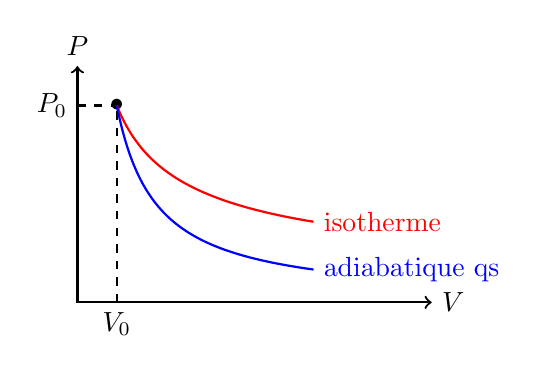
\begin{tikzpicture}[thick]
\pgfmathsetmacro{\VA}{0.5};
\pgfmathsetmacro{\PA}{2.5};

\node at (\VA,\PA) {$\bullet$};
\draw [dashed]  (0,\PA) node [left]  {$P_0$} -- (\VA,\PA);
\draw [dashed] (\VA,0) node [below] {$V_0$} -- (\VA,\PA);

\draw [red, samples=200, domain=\VA:3, variable=\V] plot (\V, {\PA * (\VA / \V)^0.5}) node [right] {isotherme};
\draw [blue, samples=200, domain=\VA:3, variable=\V] plot (\V, \PA * \VA / \V) node [right] {adiabatique \abr{qs}};

\draw [<->] (0,3) node [above] {$P$} -- (0,0) -- (4.5,0) node [right] {$V$};
\end{tikzpicture}
\end{center}
\end{figure}
\end{propriete}



\subsection{Entropie}

\begin{propriete}
L'\imp{entropie infinitésimale} $\dif S^{\text{\abr{gp}}}$ d'un \imp{\abr{gp}} est une fonction de deux variables :

\begin{itemize}
\item \tdef{fonction de $T$ et $V$} :
\[\dif S^{\text{\abr{gp}}} = C_V \frac{\dif T}{T} + nR \frac{\dif V}{V}\]

\item \tdef{fonction de $T$ et $P$} :
\[\dif S^{\text{\abr{gp}}} = C_P \frac{\dif T}{T} - nR \frac{\dif P}{P}\]

\item \tdef{fonction de $P$ et $V$} :
\[\dif S^{\text{\abr{gp}}} = C_V \frac{\dif P}{P} + C_P \frac{\dif V}{V}\]
\end{itemize}
\end{propriete}